% Chapter 12, generated by make_chapters.py from papers/Ch12_Spectral_Fibres/spectral_fibres.tex.
% Source paper: Z. Chen and R. Chen (joint)
\chapter[What a local encoder cannot see]{What a local encoder cannot see: spectral fibres of the human proteome and the representation of perturbagens}\label{chap:ch12}
\noindent{\small\emph{Joint work with Zhengyi Chen, published separately; included with the co-author's agreement.}}\par\medskip
\begin{chaptersummary}
UniPert-G2CP (Li et al., \emph{Cell} 189, 2026) represents genetic perturbagens by their protein
sequences and chemical perturbagens by ECFP4 fingerprints, and shows that its protein encoder
outperforms composition-type encoders such as pseudo amino acid composition (PseAAC). We look at
this comparison from the side of algebraic genomics, i.e.\ the combinatorics of sequences with
prescribed local content. An encoder is \emph{local of order $k$} if it depends on a sequence only
through its multiset of $k$-mers. Composition, $k$-mer composition, PseAAC with lag $\lambda\le k-1$,
and every mean-pooled convolutional encoder of window $k$ are local. So is ECFP, in the
molecular-graph sense. A local encoder is constant on the \emph{spectral fibre} of a sequence, the
set of sequences with the same $k$-mer multiset. The size of the fibre is an Eulerian-trail count,
which we compute exactly by the BEST theorem after contracting forced arcs, for all $20\,431$
reviewed human proteins. Three findings follow.
(i)~\emph{Separation is not resolution.} No two distinct human proteins share a $k$-mer spectrum
for any $k\ge2$, so every local encoder of order $\ge2$ can separate the reference proteome. Yet the
median protein shares its $3$-mer spectrum with $2^{239}$ other sequences and its $4$-mer spectrum
with $2^{19}$. The spectral resolution $\kappa$, the least $k$ beyond which the spectrum determines
the sequence, has median $5$ and exceeds $10$ for $854$ proteins.
(ii)~\emph{The unresolved order lives in duplication-driven families.} The largest $\kappa$ occur in
the hominoid-specific segmental-duplication families: NBPF, with median $\kappa=46$ and up to $951$,
then GOLGA6, NPIP and POTE. They also occur in keratin-associated proteins, collagens and mucins.
KRAB zinc-finger proteins are $3\%$ of the proteome but $41\%$ of the proteins with $\kappa>10$.
(iii)~\emph{Explicit collisions.} For $12$ human proteins we construct a different sequence, altered at
up to $15\%$ of its positions, with the same $25$-spectrum. It receives the identical $68$-dimensional
PseAAC vector (with $\lambda=24$, the setting of the UniPert benchmark) and the identical output from a
window-$25$ convolutional encoder. On the DNA side, which UniPert names as its limitation, a
strand-agnostic encoder is constant on the double-stranded reconstruction set. For bacteriophage
$\phi$X174 at $k=10$ that set has $31\,925\,753\,246\,212$ elements.
\end{chaptersummary}

\section{Introduction}\label{ch12:sec:intro}

UniPert-G2CP \cite{UniPert} is a two-stage framework for perturbation modelling. UniPert places genetic
and chemical perturbagens in one embedding space. A compound enters as an ECFP4 fingerprint
\cite{RH10}. A gene enters as its protein: mean-pooled ESM-2 embeddings \cite{ESM2} are refined by a
graph network over a Smith--Waterman similarity graph of $19\,187$ human proteins. G2CP then pretrains a
perturbation-effect predictor on CRISPR screens and fine-tunes it on compound screens. In the genetic
benchmarks (their Fig.~3B, C), UniPert is compared with ESM, OntoProtein and PseAAC. PseAAC was computed
with \texttt{propy}, $68$-dimensional, with lag $\lambda=24$; this is Chou's amphiphilic form
\cite{Chou01,Chou05}.

The question we ask is structural: \emph{what can an encoder of a given form not distinguish?} For
the family of encoders built from local statistics the answer is exact, and it is a question of
algebraic genomics. Chapters~\ref{chap:ch07}--\ref{chap:ch09} count the circular sequences that share a double-stranded
$k$-mer spectrum with a genome, by a lattice sum over the circulations of a de Bruijn double cover. For single-stranded linear sequences the same count is a single BEST
determinant \cite{BEST}. It can be computed for every protein of the human proteome, and it measures
precisely what a local encoder discards.

Section~\ref{ch12:sec:fibres} sets up local encoders and their fibres, and proves the counting formula.
Section~\ref{ch12:sec:proteome} computes fibres and spectral resolution for the proteome.
Section~\ref{ch12:sec:where} locates the unresolved order in protein families. Section~\ref{ch12:sec:mates}
constructs explicit collisions for PseAAC and for convolutional encoders. Section~\ref{ch12:sec:ecfp}
treats ECFP, and Section~\ref{ch12:sec:dna} DNA perturbagens. Section~\ref{ch12:sec:discussion} states what
the results do and do not imply for UniPert-G2CP.

\section{Local encoders and spectral fibres}\label{ch12:sec:fibres}

Let $\Sigma$ be an alphabet, $S\in\Sigma^L$ and $2\le k\le L$. The \emph{$k$-spectrum} $\spec_k(S)$ is the
multiset of the $m=L-k+1$ substrings of length $k$ of $S$. The \emph{fibre} of $S$ is
\[
F_k(S)=\{T\in\Sigma^{L}:\spec_k(T)=\spec_k(S)\},\qquad N_k(S)=|F_k(S)| .
\]
We let $F_1(S)$ be the set of rearrangements of $S$, so that $N_1(S)=L!/\prod_a n_a!$.

\begin{definition}\label{ch12:def:local}
An encoder $\phi\colon\Sigma^{*}\to\mathbb R^{d}$ is \emph{local of order $k$} if $\phi(T)=\phi(S)$
whenever $\spec_k(T)=\spec_k(S)$ and $T$, $S$ have the same first $(k-1)$-mer.
\end{definition}

The first $(k-1)$-mer is part of the definition only for bookkeeping. If the first and last
$(k-1)$-mers of $S$ differ, then every $T\in F_k(S)$ has the same first and last $(k-1)$-mers as $S$,
because they are the unique vertices of unequal in- and out-degree below.

\begin{proposition}[local encoders]\label{ch12:prop:local}
The following are local of order $k$:
\begin{enumerate}
\item composition, and $j$-mer composition for $j\le k$;
\item Chou's pseudo amino acid composition, in the original and in the amphiphilic form, with any
property scales, any weight and any lag $\lambda\le k-1$;
\item every encoder of the form $\phi(S)=\frac1n\sum_{i}f(W_i)$, where $W_1,\dots,W_n$ are the windows
of length $k$ of $S$ padded with $k-1$ sentinel symbols at each end and $f$ is arbitrary. This includes
every convolutional network of receptive field $k$ followed by mean or sum pooling.
\end{enumerate}
\end{proposition}

\begin{proof}
All three are functions of multisets of short substrings. For (1), the $j$-mer multiset is the multiset
of $j$-prefixes of the $k$-mers, together with the $j$-mers inside the last $(k-1)$-mer. For (2),
PseAAC is a function of the composition and of the correlation factors
$\tau_j=\frac1{L-j}\sum_i\Theta(S_i,S_{i+j})$, $j\le\lambda$. Here $\tau_j$ depends only on the
multiset of pairs $(S_i,S_{i+j})$, i.e.\ on the first and last letters of the $(j+1)$-mers. For (3), the
padded windows are the $k$-mers of $S$ together with windows that meet the sentinels, and those contain
only the first or the last $k-1$ letters.
\end{proof}

Being local is a property of the \emph{form} of an encoder, not of its training. A mean-pooled
transformer such as ESM-2 is not local, because attention couples all positions. An alignment
score against a reference set is not local either.

\begin{theorem}[fibre size]\label{ch12:thm:fibre}
Let $G_k(S)$ be the multigraph on the $(k-1)$-mers of $S$ with one arc $a[1..k-1]\to a[2..k]$ for each
occurrence of each $k$-mer $a$. Let $\mu(a)$ be its multiplicity, $s$ and $t$ the first and last
$(k-1)$-mers of $S$, and $d^{+}$ the out-degree. If $s\ne t$, add one arc $t\to s$. Write $\tau_s$ for
the number of spanning in-arborescences rooted at $s$, with parallel arcs counted separately. Then
\begin{equation}\label{ch12:eq:fibre}
N_k(S)\;=\;\frac{\;m^{[s=t]}\cdot\tau_s\cdot\prod_v\bigl(d^{+}(v)-1\bigr)!\;}{\prod_a\mu(a)!},
\end{equation}
where $[s=t]$ is $1$ if $s=t$ and $0$ otherwise. The whole numerator is formed before the division.
\end{theorem}

\begin{proof}
Label the arcs. The strings with $k$-spectrum $\spec_k(S)$ correspond to the Eulerian trails of
$G_k(S)$, each string to $\prod_a\mu(a)!$ labelled trails. If $s\ne t$, the trails run from $s$ to
$t$ and correspond to the Eulerian circuits of the augmented graph that begin with the added arc. By the
BEST theorem \cite{BEST} there are $\tau_s\prod_v(d^{+}(v)-1)!$ of them. If $s=t$, the trails are closed.
Every labelled circuit gives $m$ labelled closed trails, one for each starting arc, so the count is
$m\,\tau_s\prod_v(d^{+}(v)-1)!$. The factor $m$ must be applied before dividing by $\prod\mu(a)!$.
Dividing first does not give an integer, e.g.\ for $S=\mathtt{AAA}$, $k=2$.
\end{proof}

\begin{remark}[relation to the BEST theorem]\label{ch12:rem:best}
For a connected balanced multigraph $G$ with labelled arcs, the BEST theorem counts Eulerian circuits
up to rotation: $\mathrm{ec}(G)=\tau_r(G)\prod_v(d^{+}(v)-1)!$, the same for every root $r$
\cite{BEST}; this is \eqref{ch01:eq:best}. Formula~\eqref{ch12:eq:fibre} is $\mathrm{ec}$ of the closed-up graph with two corrections. The
factor $m^{[s=t]}$ restores the starting point that ``up to rotation'' forgets. The division by
$\prod_a\mu(a)!$ removes the labels, because a $k$-mer occurring $\mu$ times gives $\mu!$ labelled
copies of the same string. The same constant appears in the count
$N_{\mathrm{seq}}(c)=t(G_c)\operatorname{Loc}(G_c)/\prod_ac(a)!$ of Theorem~\ref{ch07:thm:lattice} for
circular sequences.
\end{remark}

When $s=t$, the fibre also contains the rotations that start elsewhere. The encoders of
Proposition~\ref{ch12:prop:local} are constant on the subset that starts at $s$. In the human proteome,
$s=t$ occurs for a handful of proteins and only at $k\le3$.

\begin{lemma}[forced arcs, Lemma~\ref{ch09:lem:forced}]\label{ch12:lem:forced}
If a vertex $v\ne r$ has all its out-arcs ($w\ge1$ of them) ending at one vertex $u\ne v$, then
$\tau_r(G)=w\,\tau_r(G/vu)$. Here $G/vu$ merges $v$ into $u$, deletes the arcs $v\to u$ and redirects
the arcs into $v$.
\end{lemma}

For $k\ge4$ almost every $(k-1)$-mer of a protein occurs once, and the lemma reduces $\tau$ to the
determinant of a small reduced Laplacian. The fibre moves are also classical. Two strings with the
same first $(k-1)$-mer have the same $k$-spectrum iff one is obtained from the other by a sequence of
transpositions of segments bounded by repeated $(k-1)$-mers \cite{Ukk92,Pev95}. A local encoder of
order $k$ is therefore blind to exactly those rearrangements: swaps of segments that begin and end in
repeated $(k-1)$-mers. Figure~\ref{ch12:fig:toy} shows the smallest interesting case.

\begin{figure}[t]
\centering
\resizebox{\textwidth}{!}{%
\begin{tikzpicture}[>={Stealth[length=2mm]}, font=\small,
  v/.style={draw, rounded corners=2pt, inner sep=2pt, font=\ttfamily\footnotesize},
  box/.style={draw, rounded corners=3pt, align=left, inner sep=4pt, font=\footnotesize}]
% (a) the two sequences
\node[anchor=west] at (-0.3,3.55) {\textbf{(a)}};
\node[anchor=west, font=\ttfamily] at (0.45,3.55)
  {S = MK\textbf{GS}\textcolor{blue}{AA}\textbf{GS}\textcolor{red}{WW}\textbf{GS}E};
\node[anchor=west, font=\ttfamily] at (0.45,3.05)
  {T = MK\textbf{GS}\textcolor{red}{WW}\textbf{GS}\textcolor{blue}{AA}\textbf{GS}E};
\node[anchor=west, font=\footnotesize, align=left] at (5.6,3.3)
  {the two segments between the three copies of \texttt{GS} change places;\\
   $\operatorname{spec}_3(S)=\operatorname{spec}_3(T)$, and $N_3(S)=2$: the fibre is $\{S,T\}$};
% (b) the de Bruijn graph
\node[anchor=west] at (-0.3,2.1) {\textbf{(b)}};
\node[v] (MK) at (0,0) {MK};
\node[v] (KG) at (1.2,0) {KG};
\node[v, very thick] (GS) at (2.7,0) {GS};
\node[v] (SA) at (3.7,1.0) {SA};
\node[v] (AA) at (2.7,1.7) {AA};
\node[v] (AG) at (1.7,1.0) {AG};
\node[v] (SW) at (3.7,-1.0) {SW};
\node[v] (WW) at (2.7,-1.7) {WW};
\node[v] (WG) at (1.7,-1.0) {WG};
\node[v] (SE) at (4.5,0) {SE};
\draw[->] (MK) -- (KG);
\draw[->] (KG) -- (GS);
\draw[->, blue] (GS) -- (SA);
\draw[->, blue] (SA) -- (AA);
\draw[->, blue] (AA) -- (AG);
\draw[->, blue] (AG) -- (GS);
\draw[->, red] (GS) -- (SW);
\draw[->, red] (SW) -- (WW);
\draw[->, red] (WW) -- (WG);
\draw[->, red] (WG) -- (GS);
\draw[->] (GS) -- (SE);
\draw[->, dashed] (SE.south) -- ++(0,-1.95) -| node[pos=0.25, below, font=\scriptsize] {closing arc $t\to s$} (MK.south);
\node[font=\footnotesize, align=center] at (2.3,-3.2)
  {every vertex but \texttt{GS} has one out-arc and is contracted;\\
   $d^{+}(\texttt{GS})=3$, $\tau=1$, so $N_3=\tau\,(3-1)!=2$};
% (c) encoders
\node[anchor=west] at (6.0,2.1) {\textbf{(c)}};
\node[box] (loc) at (8.6,0.8)
  {\textbf{local of order 3}\\
   composition, dipeptide composition,\\
   PseAAC with $\lambda\le2$, window-3 CNN\\
   with mean pooling:\quad $\phi(S)=\phi(T)$};
\node[box] (glob) at (8.6,-1.2)
  {\textbf{not local}\\
   ESM-2 (attention couples all positions),\\
   alignment to a reference graph:\\
   $\phi(S)$ and $\phi(T)$ may differ};
\end{tikzpicture}}
\caption{A spectral fibre in miniature. (a)~Two sequences that differ by a transposition of the segments
between three copies of the repeated $2$-mer \texttt{GS}. (b)~Their common de Bruijn graph for $k=3$. The
fibre size follows from Theorem~\ref{ch12:thm:fibre} after contracting forced arcs (Lemma~\ref{ch12:lem:forced}).
(c)~Every local encoder of order $3$ assigns them the same vector. In the human proteome the same
mechanism acts on repeat copies $25$ residues long and longer (Table~\ref{ch12:tab:mates}).}\label{ch12:fig:toy}
\end{figure}

\begin{definition}\label{ch12:def:kappa}
The \emph{spectral resolution} of $S$ is $\kappa(S)=\min\{k:N_{k'}(S)=1\text{ for all }k'\ge k\}$.
It is at most two more than the length of the longest repeated substring of $S$.
\end{definition}

\section{The human proteome}\label{ch12:sec:proteome}

We take the $20\,431$ reviewed human entries of UniProt \cite{UniProt}, with $11\,418\,237$ residues,
median length $415$ and maximum $34\,350$ (titin). For every protein and every $k$ from $1$ up to the
point where no $(k-1)$-mer repeats, we compute $N_k$ by Theorem~\ref{ch12:thm:fibre} and
Lemma~\ref{ch12:lem:forced}. The computation is exact whenever the contracted Laplacian has order at most
$150$. Larger orders occur only at small $k$ in long proteins, where $\log_2N_k$ is in the thousands.
There the determinant is taken in floating point, and the logarithms of the factorials come from
$\log\Gamma$. Against exact values on $200$ random sequences, the worst relative error of that path
is $6.5\cdot10^{-16}$. The formula itself is checked against exhaustive enumeration in $21\,187$ cases
(alphabets of size $2$--$4$, lengths up to $12$). The contraction is checked against the full
determinant on $400$ random sequences. The whole run takes $18$ minutes on $16$ processes.

\begin{table}[t]
\centering\small
\begin{tabular}{rrrrl}
\toprule
$k$ & proteins with $N_k>1$ & share & median $\log_2N_k$ & largest $\log_2N_k$\\
\midrule
1 & 20\,431 & 100.00\% & 1628.4 & 140\,656.7 (TTN)\\
2 & 20\,422 & 99.96\% & 1080.5 & 136\,673.4 (TTN)\\
3 & 20\,357 & 99.64\% & 239.4 & 114\,168.6 (TTN)\\
4 & 18\,391 & 90.02\% & 18.9 & 55\,107.2 (TTN)\\
5 & 9\,504 & 46.52\% & 0 & 13\,489.5 (TTN)\\
6 & 3\,445 & 16.86\% & 0 & 6\,247.9 (MUC3B)\\
8 & 1\,346 & 6.59\% & 0 & 3\,715.5 (MUC3B)\\
10 & 854 & 4.18\% & 0 & 2\,252.5 (MUC3B)\\
12 & 614 & 3.01\% & 0 & 1\,269.2 (MUC3B)\\
16 & 327 & 1.60\% & 0 & 404.2 (MUC4)\\
20 & 194 & 0.95\% & 0 & 255.4 (MUC2)\\
25 & 114 & 0.56\% & 0 & 164.2 (MUC2)\\
30 & 81 & 0.40\% & 0 & 108.8 (MUC2)\\
40 & 50 & 0.25\% & 0 & 63.1 (MUC2)\\
50 & 37 & 0.18\% & 0 & 37.2 (NBPF20)\\
\bottomrule
\end{tabular}
\caption{Spectral fibres of the $20\,431$ reviewed human proteins. $N_k$ is the number of sequences
with the same $k$-mer multiset.}\label{ch12:tab:fibres}
\end{table}

Table~\ref{ch12:tab:fibres} summarizes the fibres. From $k=5$ on, the median of $\log_2N_k$ is $0$, i.e.\
$N_k=1$: more than half of all human proteins ($53.5\%$) are already determined by their $5$-mer
spectrum, and the median describes the resolved majority. The tail is what matters, and it is in the
second and last columns (Figure~\ref{ch12:fig:resolution}a). The spectral resolution has median $\kappa=5$
(Figure~\ref{ch12:fig:resolution}b). Its
$90\%$ and $99\%$ quantiles are $7$ and $20$, and its maximum is $951$ (NBPF20). The cumulative shares
are:
\begin{gather*}
\kappa\le4:\ 10.0\%,\qquad \kappa\le5:\ 53.5\%,\qquad \kappa\le6:\ 83.1\%,\\
\kappa\le8:\ 93.4\%,\qquad \kappa\le10:\ 95.8\%,\qquad \kappa\le25:\ 99.4\%.
\end{gather*}

\begin{figure}[t]
\centering
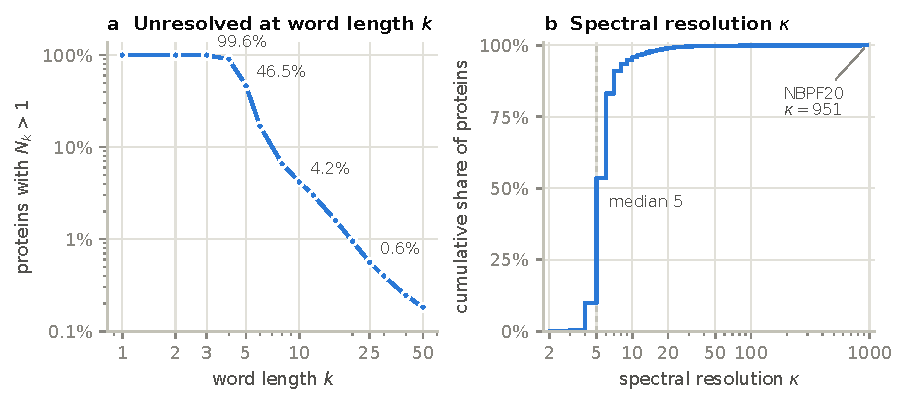
\includegraphics[width=\textwidth]{../papers/Ch12_Spectral_Fibres/fig_resolution.pdf}
\caption{Spectral resolution of the $20\,431$ reviewed human proteins. (a)~Share of proteins whose
$k$-spectrum does not determine them ($N_k>1$), on logarithmic axes. (b)~Cumulative distribution of the
spectral resolution $\kappa$. The dashed line marks the median, $5$.}\label{ch12:fig:resolution}
\end{figure}

\paragraph{Separation is not resolution.} Among the $20\,353$ distinct sequences, exactly one pair shares
its amino acid composition. No two share their $k$-spectrum for $k=2,3,4$. So even dipeptide
composition separates every protein of the reference proteome from every other, and nothing in the
\emph{training set} of a protein encoder forces it to look further. What the reference set does not
contain is the fibre: at $k=3$ the median protein has $2^{239}$ spectral twins, and at $k=4$ still
$2^{19}$. Those are exactly the inputs on which out-of-distribution generalization is tested:
rearranged, recombined or unseen sequences. On them a local encoder of order $3$ or $4$ is constant
by construction, whatever it learned. Separating a finite reference set and resolving sequence
space are different properties, and benchmarks on the reference set test only the first.

\paragraph{Proteins named in UniPert-G2CP.} Table~\ref{ch12:tab:named} lists proteins that appear in the
UniPert-G2CP analyses: the unseen single-gene targets CEP55, AURKA and AURKB, the combination
CBL$+$CNN1, the kinesin/FOXM1 example, PD-1/PD-L1, the GABA$_{\mathrm A}$ receptor, and ESR1. All
have $\kappa$ between $5$ and $11$. The kinesin CENPE is the least resolved, with $226$ bits of
unresolved order at $k=5$.

\begin{table}[t]
\centering\small
\begin{tabular}{lrrrrrr}
\toprule
protein & $L$ & $\kappa$ & $\log_2N_3$ & $\log_2N_4$ & $\log_2N_5$ & $\log_2N_6$\\
\midrule
ESR1 & 595 & 5 & 408.2 & 33.7 & 0 & 0\\
CEP55 & 464 & 6 & 361.9 & 43.5 & 1.6 & 0\\
AURKA & 403 & 5 & 234.1 & 18.9 & 0 & 0\\
AURKB & 344 & 5 & 152.2 & 6.6 & 0 & 0\\
CBL & 906 & 7 & 878.8 & 90.8 & 15.2 & 1.6\\
CNN1 & 297 & 7 & 109.1 & 13.1 & 5.0 & 1.6\\
CENPE & 2701 & 11 & 5298.0 & 1352.8 & 226.3 & 48.3\\
FOXM1 & 763 & 6 & 773.9 & 78.3 & 3.0 & 0\\
PDCD1 (PD-1) & 288 & 5 & 128.3 & 9.2 & 0 & 0\\
CD274 (PD-L1) & 290 & 6 & 92.0 & 6.2 & 1.0 & 0\\
GABRA1 & 456 & 5 & 265.1 & 19.4 & 0 & 0\\
\bottomrule
\end{tabular}
\caption{Proteins discussed in UniPert-G2CP \cite{UniPert}. $\log_2N_k$ is the number of bits of
order that a local encoder of order $k$ cannot see.}\label{ch12:tab:named}
\end{table}

\section{Where the unresolved order lives}\label{ch12:sec:where}

Fibres grow with length at small $k$: a long protein repeats many short words by chance, so
$\log_2N_3/L$ is largest for titin ($3.32$ bits per residue), the mucins, nesprins and plakins. The
spectral resolution does not grow with length in this way. It is large only if the protein contains
long repeats that interleave or recur, so it is the family-level statistic. Figure~\ref{ch12:fig:families}b
shows this directly. Proteins of every length reach $\kappa\le10$, while the large values belong to
particular families at moderate lengths.

\begin{figure}[t]
\centering
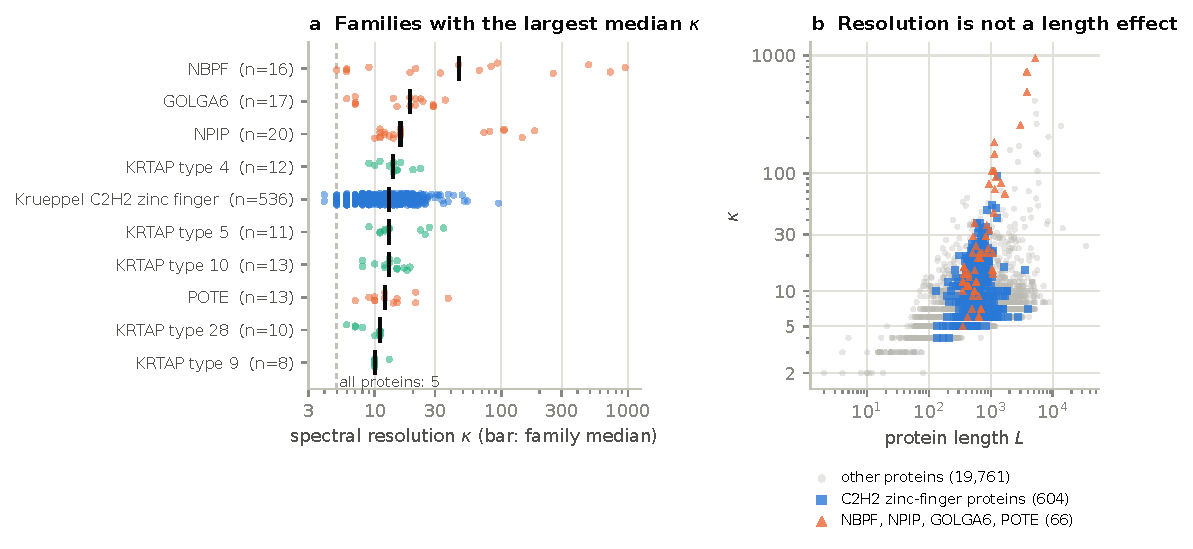
\includegraphics[width=\textwidth]{../papers/Ch12_Spectral_Fibres/fig_families.pdf}
\caption{Where the unresolved order lives. (a)~The ten families (at least eight members) with the largest
median $\kappa$. Each dot is a protein, and the bar is the family median. Orange: hominoid/primate-specific
segmental-duplication families; blue: Krueppel C2H2 zinc-finger proteins; green: keratin-associated
proteins. The dashed line is the proteome median. (b)~$\kappa$ against protein length for all proteins.
The two highlighted groups are shown in their own colours and marker shapes.}\label{ch12:fig:families}
\end{figure}

\begin{table}[t]
\centering\small
\begin{tabular}{>{\raggedright\arraybackslash}p{0.3\textwidth}rr>{\raggedright\arraybackslash}p{0.36\textwidth}}
\toprule
family (UniProt) & members & median $\kappa$ & origin of the repeats\\
\midrule
NBPF & 16 & 46 & Olduvai (DUF1220) domain amplification, hominoid-specific\\
GOLGA6 & 17 & 19 & segmental duplication, hominoid-specific\\
NPIP & 20 & 16 & segmental duplication, hominoid-specific\\
KRTAP type 4 & 12 & 14 & cysteine-rich pentapeptide repeats\\
Krueppel C2H2 zinc finger & 536 & 13 & tandem C2H2 fingers\\
KRTAP types 5, 10 & 11, 13 & 13 & cysteine-rich repeats\\
POTE & 13 & 12 & segmental duplication, primate-specific\\
KRTAP types 28, 9 & 10, 8 & 11, 10 & cysteine-rich repeats\\
collagens (fibrillar, FACIT) & 11, 9 & 10 & Gly-X-Y triplets\\
\midrule
all proteins & 20\,431 & 5 & \\
\bottomrule
\end{tabular}
\caption{Families with at least eight members, ranked by median spectral resolution.}\label{ch12:tab:fam}
\end{table}

Table~\ref{ch12:tab:fam} ranks families by median $\kappa$. The top of the list is not a random sample of
repetitive proteins. The first three families and POTE arose by segmental duplication in the hominoid
lineage. The NBPF proteins carry the Olduvai (DUF1220) domain, whose copy number expanded
dramatically in humans \cite{OBl12}, and NBPF20 has $\kappa=951$. The next group consists of tandem-repeat
families whose repeat units are identical or nearly identical: keratin-associated proteins,
collagens, and the Krueppel C2H2 zinc-finger proteins. The latter are dominated by the KRAB
zinc-finger proteins, which expanded with the transposable elements they control \cite{Imb17}.

The zinc fingers are the clearest case. The $604$ proteins whose family annotation contains
``C2H2-type zinc-finger'' are $3.0\%$ of the proteome. Yet $348$ of them have $N_{10}>1$, i.e.\
$41\%$ of the $854$ proteins that remain unresolved at $k=10$. ZNF91 and ZNF208, which have
$\kappa=51$ and $95$, are typical. These are also the proteins whose \emph{specificity} lies in which
finger sits where: the DNA motif a KZFP recognizes is read off the order of its fingers.
UniPert's Fig.~2G singles out the zinc-finger family as one its embedding clusters well. That is
consistent with our finding: a composition-type encoder sees these proteins as nearly
interchangeable, while an alignment graph and a contextual language model do not.

\section{Explicit collisions}\label{ch12:sec:mates}

For $114$ human proteins $N_{25}>1$, so PseAAC with $\lambda=24$, the setting of the UniPert
benchmark, is not injective on their fibres. To make this concrete, we take $12$ of them spread over
lengths $187$--$2078$. For each, we draw a random Eulerian trail with the same start by Hierholzer's
algorithm, and keep it if it spells a different sequence. For every pair we then check exactly
(in rational arithmetic) three things: the $25$-spectra coincide; the $68$-dimensional amphiphilic
PseAAC vectors coincide; and the outputs of a random $8$-channel integer convolutional network with
window $25$ and mean pooling coincide. The PseAAC vectors were computed with the Kyte--Doolittle and
Hopp--Woods scales, but by Proposition~\ref{ch12:prop:local} the scales are irrelevant. The pairs are far
from identical (Table~\ref{ch12:tab:mates}). Figure~\ref{ch12:fig:mates} shows where they differ. The changes
come in contiguous blocks, the transposed segments, and in the zinc-finger proteins these blocks span
several fingers.

\begin{figure}[t]
\centering
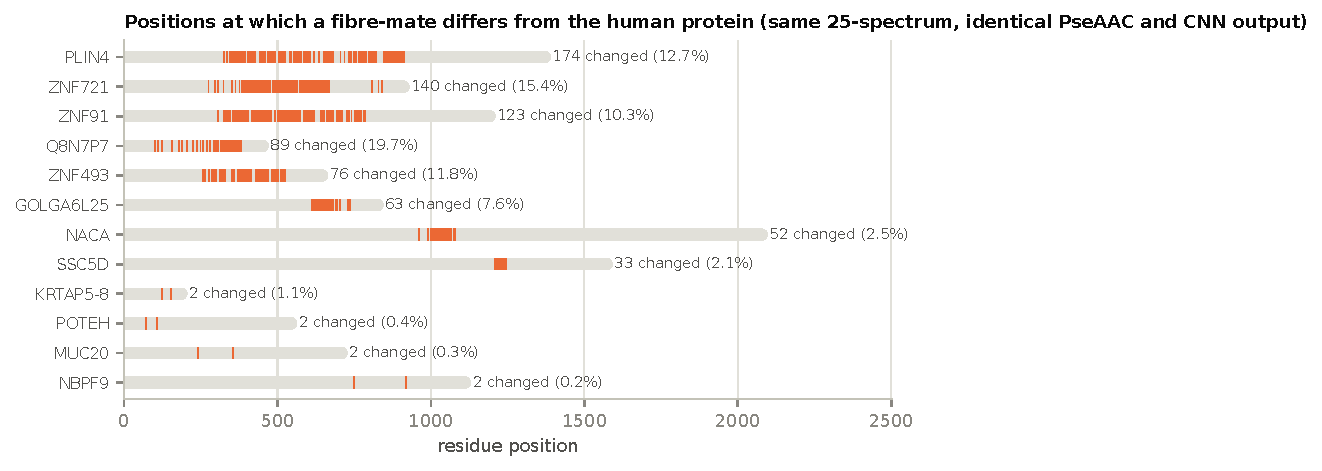
\includegraphics[width=\textwidth]{../papers/Ch12_Spectral_Fibres/fig_mates.pdf}
\caption{The twelve fibre-mates of Table~\ref{ch12:tab:mates}. Each grey bar is a human protein, and orange
marks the positions at which its fibre-mate differs. Each pair has the same $25$-spectrum, the identical
$68$-dimensional PseAAC vector and the identical output from a window-$25$ convolutional encoder.}\label{ch12:fig:mates}
\end{figure}

\begin{table}[t]
\centering\small
\begin{tabular}{lrrrc}
\toprule
protein & $L$ & positions changed & SW$(S,T)/$SW$(S,S)$ & PseAAC, CNN\\
\midrule
KRTAP5-8 & 187 & 2 (1.1\%) & 0.984 & identical\\
Q8N7P7 & 452 & 89 (19.7\%) & 0.814 & identical\\
POTEH & 545 & 2 (0.4\%) & 0.994 & identical\\
ZNF493 & 646 & 76 (11.8\%) & 0.824 & identical\\
MUC20 & 709 & 2 (0.3\%) & 0.996 & identical\\
GOLGA6L25 & 826 & 63 (7.6\%) & 0.944 & identical\\
ZNF721 & 911 & 140 (15.4\%) & 0.769 & identical\\
NBPF9 & 1111 & 2 (0.2\%) & 0.997 & identical\\
ZNF91 & 1191 & 123 (10.3\%) & 0.846 & identical\\
PLIN4 & 1371 & 174 (12.7\%) & 0.815 & identical\\
SSC5D & 1573 & 33 (2.1\%) & 0.981 & identical\\
NACA & 2078 & 52 (2.5\%) & 0.986 & identical\\
\bottomrule
\end{tabular}
\caption{A human protein $S$ and a different sequence $T$ with the same $25$-spectrum and the same
start. SW is a Smith--Waterman local alignment score (match $2$, mismatch $-1$, gap $-2$). PseAAC is the $68$-dimensional amphiphilic form with $\lambda=24$; CNN is an
$8$-channel window-$25$ integer network with mean pooling.}\label{ch12:tab:mates}
\end{table}

The pairs changed at two positions deserve a remark. There, two copies of a repeat unit differ at
one residue each, and the fibre-mate swaps the two variants between the copies. A local encoder of
order $25$ cannot tell \emph{which copy carries which variant}. In the zinc-finger pairs, whole
fingers change places ($10$--$15\%$ of positions). The alignment score drops to $0.77$--$0.85$ of the
self-score, so the two sequences are far apart for an alignment-based encoder, and yet they are
indistinguishable for PseAAC.

\section{The chemical side: ECFP}\label{ch12:sec:ecfp}

ECFP is the molecular analogue of a $k$-mer spectrum \cite{RH10}. After $r$ rounds, each atom carries
an identifier of its radius-$r$ environment. The fingerprint is the \emph{set} of identifiers of all
atoms, hashed into $2048$ bits, with multiplicities discarded in the binary form that UniPert uses
($r=2$). It is therefore local in the graph sense. Molecules with the same radius-$2$ environment
set receive the same fingerprint. The refinement is the Weisfeiler--Lehman colour refinement, whose
blind spots (regular and symmetric graphs, rings of equal local structure) are well
documented \cite{XHLJ19}. Binarization makes the fibre larger than its sequence counterpart, since it
forgets how many atoms share an environment. The radius also fixes a horizon. A radius-$2$
environment reaches two bonds from its centre, so no single identifier spans more than four bonds.
Two molecules that assemble the same environments into different long-range arrangements (the
order of substituents along a chain, the placement of equal units around a macrocycle) therefore
lie in the same fibre. This is the exact analogue of a transposition between repeated
$(k-1)$-mers. The default ECFP also carries no stereochemistry, so stereoisomers (enantiomers,
\emph{cis}/\emph{trans} isomers) always share a fingerprint unless chirality flags are switched on.
Both are \emph{molecular fibres} in the sense of this chapter: sets of distinct perturbagens that a local
encoder cannot tell apart, whatever it was trained on. We do not compute molecular fibres here. We note only
that in UniPert-G2CP both perturbagen types would have been local, had the protein encoder been
PseAAC: the gain on the genetic side comes precisely from giving up locality.

\section{DNA perturbagens and the double cover}\label{ch12:sec:dna}

UniPert-G2CP names as its limitation that genetic perturbations outside protein-coding genes cannot
be represented, and points to DNA language models. DNA brings one more symmetry. A regulatory
element, or a CRISPR target, has no preferred strand, so a DNA encoder that is to be strand-agnostic
must satisfy $\phi(S)=\phi(\bar S)$ for the reverse complement $\bar S$. A local encoder with this
property depends only on the \emph{double-stranded} spectrum $\spec_k(S)+\spec_k(\bar S)$. Its fibre
is the set $\DS(S,k)$ of double-stranded reconstructions.

\begin{proposition}\label{ch12:prop:ds}
A strand-agnostic local encoder of order $k$ is constant on $\DS(S,k)$. For circular $S$,
\[
|\DS(S,k)|=\sum_{f}N_{\mathrm{seq}}\Bigl(\tfrac{m+f}{2}\Bigr),
\]
the sum running over the points $f$ of the $(-1)$-eigenlattice of the reverse-complement involution
on the circulations of the double cover $D_k$, inside the box $|f|\le m$ (Theorem~\ref{ch07:thm:lattice}).
\end{proposition}

This fibre is not given by a single determinant. It is a lattice sum of determinants, and it is
much harder to compute. For the $5\,386$-bp genome of $\phi$X174 at $k=10$, the lattice has rank $48$
and the box has $2\,481\,687\,900$ points, of which $909\,103\,210$ have connected support (Chapter~\ref{chap:ch08}).
The number of double-stranded reconstructions is
\[
|\DS(\phi\mathrm{X}174,10)|=31\,925\,753\,246\,212
\]
(Chapter~\ref{chap:ch09}). A strand-agnostic local DNA encoder of window $10$ assigns all of them the same
vector. The design choice ``make the encoder reverse-complement invariant'' is sound, but it has a
price. For local encoders that price is exactly the passage from a sequence fibre to a
double-stranded fibre.

\section{What this does and does not imply}\label{ch12:sec:discussion}

\begin{table}[t]
\centering\small
\renewcommand{\arraystretch}{1.25}
\begin{tabular}{>{\raggedright\arraybackslash}p{0.33\textwidth}>{\raggedright\arraybackslash}p{0.58\textwidth}}
\toprule
UniPert-G2CP & what the fibre analysis adds\\
\midrule
UniPert outperforms PseAAC, ESM, OntoProtein in genetic OOD tasks & PseAAC ($\lambda=24$) is constant on
$25$-fibres: provably identical vectors for $12$ explicit human protein pairs differing at up to $15\%$
of positions; $114$ proteins have non-trivial $25$-fibres\\
sequence-based encoders ``risk losing local information'' & composition-type encoders lose
\emph{global order}, not local content: median $2^{239}$ twins at $k=3$, $2^{19}$ at $k=4$; median
resolution $\kappa=5$\\
reference set of $19\,187$ proteins & every local encoder of order $\ge2$ already separates the reference
proteome; separation of the reference set is not evidence of resolution\\
zinc-finger family clustered well (Fig.~2G) & KZFPs are $3\%$ of proteins but $41\%$ of those with
$\kappa>10$; their function is in finger order, which local encoders cannot see\\
ESR1 domains and mutants (Fig.~6) & $\kappa(\mathrm{ESR1})=5$; a point substitution changes at most $k$
of the $k$-mers, and it is visible to any local encoder of order $\le\kappa$\\
ECFP4 for compounds & ECFP is a local (radius-$2$, binarized) encoder; its blind spots are those of
Weisfeiler--Lehman refinement\\
limitation: non-coding perturbations & a strand-agnostic local DNA encoder is constant on the
double-stranded reconstruction set, $3.19\cdot10^{13}$ sequences for $\phi$X174 at $k=10$\\
\bottomrule
\end{tabular}
\caption{The results of this chapter set against the corresponding statements of UniPert-G2CP.}\label{ch12:tab:vs}
\end{table}

Table~\ref{ch12:tab:vs} sets our results against the statements of UniPert-G2CP. Three limitations
should be stated plainly.

First, a fibre is a set of \emph{sequences}, not of proteins. Most fibre members are not
biologically plausible, and a model trained on real proteins may never meet them. The fibres that
matter are those reached by real processes, and here one must distinguish. Exon skipping, exon
duplication and domain deletion change the $k$-mer content: they add or remove $k$-mers. So they
move a sequence \emph{out of} its fibre, and a local encoder does register them. What a local encoder
cannot register is a change of order at constant content. Such changes include: gene conversion or
unequal crossing-over that swaps variants between repeat copies; a variant assigned to the wrong copy
of a repeat; and a reordering of identical or near-identical units, such as fingers in a KZFP, Olduvai
domains in an NBPF protein, or cysteine-rich repeats in a KRTAP. These are the transpositions of
Section~\ref{ch12:sec:fibres}, and they are concentrated in the families of Table~\ref{ch12:tab:fam}. Whether
such events have phenotypic consequences that a perturbation model should predict is open. When they
do, a local encoder cannot predict them.

Second, we have not evaluated UniPert, ESM or any trained model. Our statements about PseAAC and
convolutional encoders are theorems about their form. The comparison with UniPert's benchmark offers
a mechanism consistent with their ranking, not a test of it. Such a test is easy to set up: a
\emph{fibre-mate benchmark}. It would pair each protein with a sequence from its $k$-fibre (for
example, a repeat-copy swap), and ask whether an encoder separates the pair and whether a predictor
assigns them different effects.

Third, the spectral resolution measures what is \emph{invisible} to local statistics, not what is
\emph{relevant} to a phenotype. Whether finger order in a KZFP changes a perturbation phenotype is a
biological question. Our analysis says only that a local encoder cannot represent the answer.

\section*{Data and code availability}
\texttt{spectral\_fibres.py} (Python 3.10+, standard library; \texttt{numpy} only for the
floating-point determinants) downloads the reviewed human proteome from UniProt. It then runs the
five checks (formula, contraction, proteome, collisions, fibre-mates) and writes the per-protein
results (\texttt{fibre\_results.json}). The transcript is \texttt{spectral\_fibres\_output.txt}. The
double-stranded count of Section~\ref{ch12:sec:dna} is reproduced by the ancillary files of Chapter~\ref{chap:ch09}.
